\section{Interpolation and Extrapolation} \label{sec:Interpolation and Extrapolation}

Let's say that we have a coarsely-sampled function that we would like to re-sample at a higher rate. Suppose that you have the data shown in Figure \ref{fig:Coarsely-sampled Function}, which is sampled at 10 samples per second. Instead, you want to sample at 100 samples per second, or more. Several different interpolation methods are shown in Figure \ref{fig:Interpolated Function}.

\begin{figure}[htp]
    \centering
    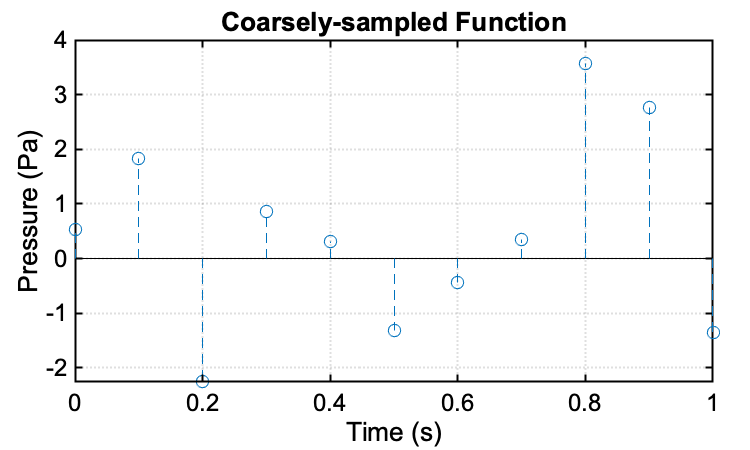
\includegraphics[width = 5 in]{Chapters/Computational Methods/Figures/Coarsely-sampled Function.png}
    \caption{A coarsely-sampled function.}
    \label{fig:Coarsely-sampled Function}
\end{figure}

\begin{figure}[htp]
    \centering
    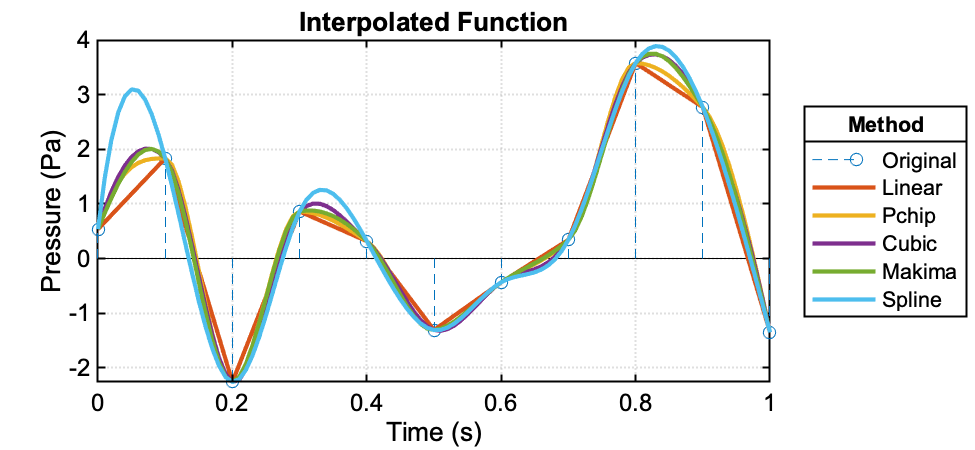
\includegraphics[width = 6.5 in]{Chapters/Computational Methods/Figures/Interpolated Function.png}
    \caption{The interpolated function shown for several interpolation methods.}
    \label{fig:Interpolated Function}
\end{figure}

\subsection{Spectral Effects of Interpolation in the Time Domain}

Looking at the different varieties of interpolated signals in Figure \ref{fig:Interpolated Function}, it makes me wonder, what happens to the frequency content when the function is interpolated to give a higher sampling frequency? To further investigate this question, I created some normally-distributed random noise sampled at 12.6 kHz. The waveform is shown in Figure \ref{fig:Randomly-Distributed Gaussian Noise}. I then interpolated the waveform up to a sampling frequency of 51.2 kHz using each of the methods. Using these interpolated waveforms, I calculated the autospectral densities and then the one-third octave band SPL spectra.

The spectra contain the surprising result that the interpolation methods all produce similar results to the original waveform. Evidently very little, if any, higher-frequency data can be created by interpolating between time series data points.

\begin{figure}[htp]
    \centering
    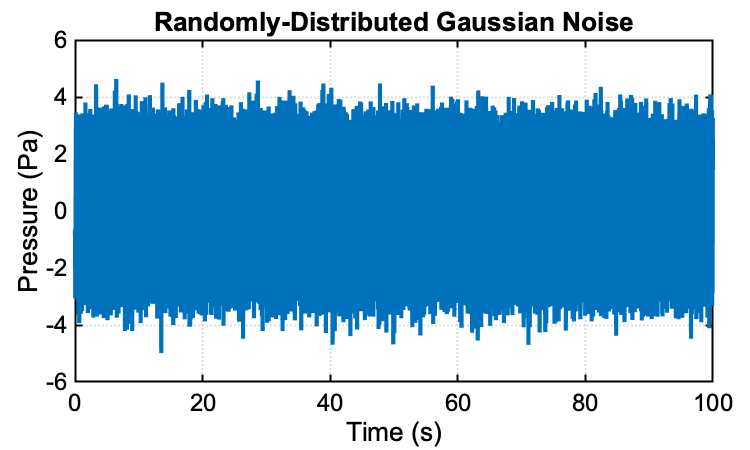
\includegraphics[width = 5 in]{Chapters/Computational Methods/Figures/Randomly-Distributed Gaussian Noise.png}
    \caption{Randomly-distributed gaussian noise.}
    \label{fig:Randomly-Distributed Gaussian Noise}
\end{figure}

\begin{figure}[htp]
    \centering
    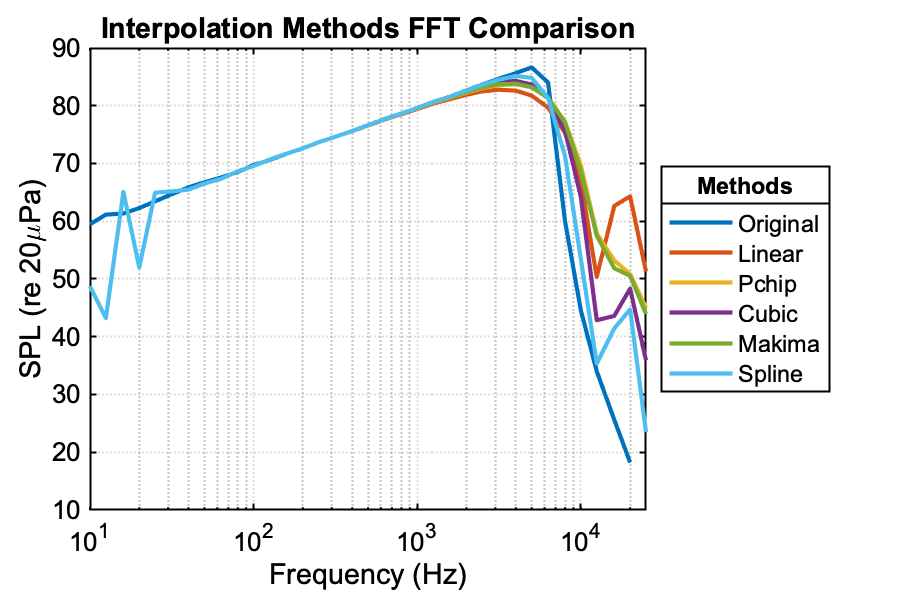
\includegraphics[width = 6 in]{Chapters/Computational Methods/Figures/Interpolation Methods FFT Comparison.png}
    \caption{The OTO band spectra for the signal before and after being interpolated by each of the shown methods.}
    \label{fig:Interpolation Methods FFT Comparison}
\end{figure}